\subsection{Period 1: \change{A very well delimited} detached haze Layer during the Northern Winter (2004-2008) - $L_s=\ang{300}-\ang{340}$}

At its arrival in the Saturnian system in 2004, Cassini observed a single detached haze layer at 500 km altitude
(Fig.~\ref{fig:dhl_2004_2008}a) similar to the one observed at 350 km by Voyager 24 years before
\citep{Smith1981}. At that moment, Titan was two years after the winter solstice in the northern hemisphere, at $L_s=\ang{300}$.
With Cassini, we see that, in the southern hemisphere, the haze layer was completely detached from the main haze layer.
The haze extinction was at least one order of magnitude smaller inside the depleted zone (470 km) than in the main and
the detached haze layers (below 450 and at 500 km respectively).
Between the equator and up to about \ang{60}N it presented a local depletion in extinction
of a factor 10. There, the separation with the main haze is not as distinct as in the south, but is still sufficiently significant to
defined a detached haze layer.
The altitude of the depletion zone decreased by about 50 km between latitude \ang{30}N  and \ang{60}N.
The detached haze layer merged with the polar hood beyond \ang{60}N. This description of the detached haze layer at
the beginning of Cassini mission is very consistent with the results obtained from stellar occultation in 2003 \citep{Sicardy2006}.
Throughout the period 2004-2008 the detached haze layer was quite stable in shape and  altitude, with a maximum of extinction
at $500 \pm 20$ km. The top of the main haze layer was located around $450 \pm 20$ km below \ang{30}N and dropped
by 50 km between \ang{30} and \ang{60}N.

\begin{figure*}[!ht]
\plotone{Fig/Lat_beta-2004_2008}
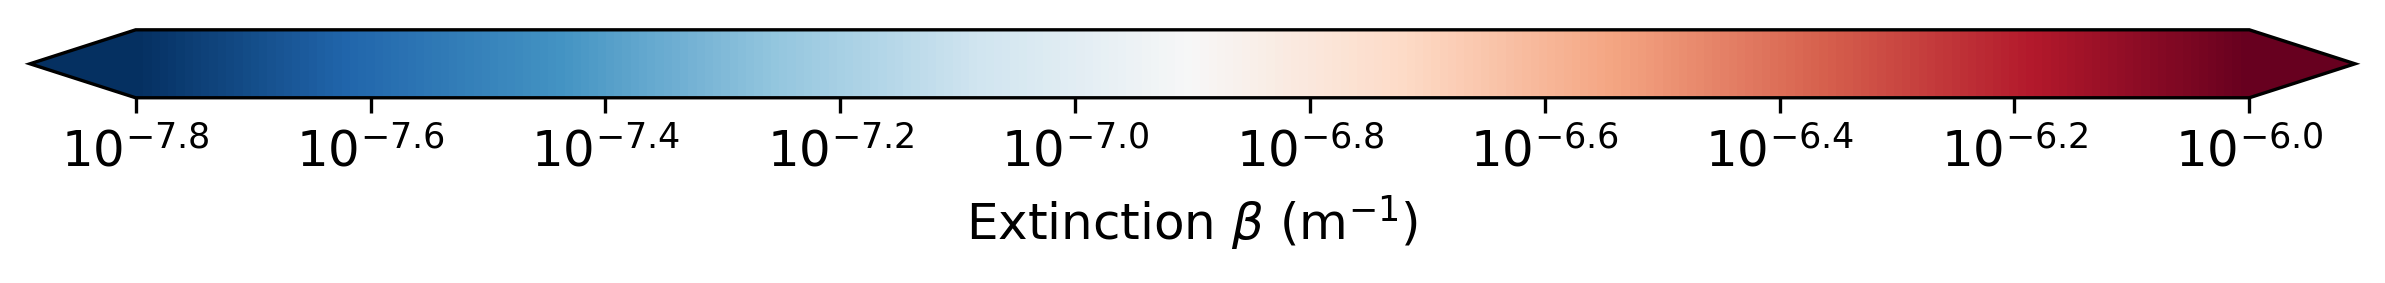
\includegraphics[width=.5\textwidth]{Fig/Extinction_colorbar}
\caption{Latitudinal haze extinction profile ($\beta$) retrieved for 6 images taken between 2004 and 2008
($L_s=\ang{300}-\ang{340}$) showing a stable DHL at $500 \pm 20$ km altitude.
The color schema is fixed for all the figures to make direct comparison
between the different panels. The seasonal solar longitude ($L_s$) and the observation phase angle are
also provided in each panel.}
\label{fig:dhl_2004_2008}
\end{figure*}

However, there are noticeable variations in haze extinction. During several months, the
detached haze remained stable, but in December 2004 (Fig.~\ref{fig:dhl_2004_2008}b),
the detached haze layer extinction was found to be a factor of 10 lower than previously at almost all latitudes south
of \ang{30}N, and about half a decade above \ang{30}N. The polar hood and the main haze do not show a similar decrease.
In the following periods, (Fig.~\ref{fig:dhl_2004_2008}c, d and e),
the detached haze was partially restored, but not with the same amount of extinction as before. Only observations in
2007 (Fig.~\ref{fig:dhl_2004_2008}f) show extinctions in the detached haze layer comparable to those seen before
the decrease. We note that the decrease of extinction below 370 km in the polar hood above \ang{50}N
(Fig.~\ref{fig:dhl_2004_2008}e) is at the limit of sensitivity of the UV filter. The stability of the large-scale
structure of the detached haze layer is related to the steady state of the large-scale circulation during all the winter.
The observation of October 2007 (Fig.~\ref{fig:dhl_2004_2008}f) is the last view that we have of this stable state
before the seasonal turnover.

During this period, the detached haze also has a strong layering with, at some latitudes, distinct decks which are not
continuous and rather appear as foliation. This feature is more pronounced in some observations, for instance from
June 2005 to May 2006, but does not shows up in October 2007, except marginally beyond \ang{30}N. The foliated detached
haze layer has a larger geometrical thickness than before December 2004.

As we will see in the \textbf{section 4}, the detached haze layer exhibits some longitudinal or diurnal variability
that limits our ability to interpret details of features observed in single images. The small-scale features
could depend on the local short-term dynamics such as initia-gravity waves.
